%!TEX TS-program = xelatex
%!TEX encoding = UTF-8 Unicode
% Awesome CV LaTeX Template
%
% This template has been downloaded from:
% https://github.com/posquit0/Awesome-CV
%
% Author:
% Claud D. Park <posquit0.bj@gmail.com>
% http://www.posquit0.com
%
% Template license:
% CC BY-SA 4.0 (https://creativecommons.org/licenses/by-sa/4.0/)
%


%%%%%%%%%%%%%%%%%%%%%%%%%%%%%%%%%%%%%%
%     Configuration
%%%%%%%%%%%%%%%%%%%%%%%%%%%%%%%%%%%%%%
%%% Themes: Awesome-CV
\documentclass[]{awesome-cv}
\usepackage{textcomp}
\usepackage{graphicx}
%%% Override a directory location for fonts(default: 'fonts/')
\fontdir[fonts/]

%%% Configure a directory location for sections
\newcommand*{\sectiondir}{resume/}

%%% Override color
% Awesome Colors: awesome-emerald, awesome-skyblue, awesome-red, awesome-pink, awesome-orange
%                 awesome-nephritis, awesome-concrete, awesome-darknight
%% Color for highlight
% Define your custom color if you don't like awesome colors
\colorlet{awesome}{awesome-red}
%\definecolor{awesome}{HTML}{CA63A8}
%% Colors for text
%\definecolor{darktext}{HTML}{414141}
%\definecolor{text}{HTML}{414141}
%\definecolor{graytext}{HTML}{414141}
%\definecolor{lighttext}{HTML}{414141}

%%% Override a separator for social informations in header(default: ' | ')
%\headersocialsep[\quad\textbar\quad]
    \begin{document}
%%%%%%%%%%%%%%%%%%%%%%%%%%%%%%%%%%%%%%
%     Profile
%%%%%%%%%%%%%%%%%%%%%%%%%%%%%%%%%%%%%%
\begin{minipage}[b]{0.66666\textwidth}
\begin{center}
	\headerfirstnamestyle{Adrián} \headerlastnamestyle{Arroyo Calle} \\
	\vspace{2mm}
	{\faEnvelope\ adrian.arroyocalle@gmail.com} | {\faMobile\ +34 602 133 602} \newline {\faMapMarker\ Valladolid, Spain} {\faLink\ \url{http://adrianistan.eu}}
\end{center}
\end{minipage}
% FOTO
%\begin{minipage}[b]{0.33333\textwidth}
%	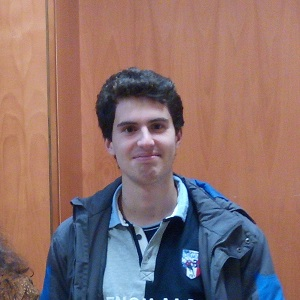
\includegraphics[width=0.8\textwidth]{stallman.jpg}
%\end{minipage}

%%%%%%%%%%%%%%%%%%%%%%%%%%%%%%%%%%%%%%
%     Education
%%%%%%%%%%%%%%%%%%%%%%%%%%%%%%%%%%%%%%
\cvsection{Educación}
\begin{cventries}
	\cventry
	{Graduado en Ingeniería Informática}
	{Universidad de Valladolid}
	{Valladolid, España}
	{2016-2020}
	{}
\end{cventries}

\vspace{-2mm}
%%%%%%%%%%%%%%%%%%%%%%%%%%%%%%%%%%%%%%
%     Experience
%%%%%%%%%%%%%%%%%%%%%%%%%%%%%%%%%%%%%%
\cvsection{Experiencia}
\begin{cventries}
	\cventry
	{Backend Developer}
	{Telefónica}
	{Boecillo, España}
	{Julio 2020 - Presente}
	{\begin{cvitems}
		\item {LivingApps Maker}
		\item {Python, FastAPI, React, TypeScript}
	\end{cvitems}}
	\cventry
	{Becario}
	{Telefónica I+D}
	{Boecillo, España}
	{Julio 2019 - Junio 2020}
	{\begin{cvitems}
		\item {4th Platform}
		\item {GitOps, Kubernetes, Docker}
	\end{cvitems}
	}
\end{cventries}
\cvsection{Destrezas}
\begin{cventries}
	\cventry
	{}
	{\def\arraystretch{1.15}{\begin{tabular}{ l l }
		Lenguajes de programación:  & {\skill{ Rust, C, Python, Java, JavaScript, SQL, Prolog}} \\
		Idiomas:  & {\skill{ Español (nativo), Inglés ( FIRST B2)}} \\
		Software: & {\skill{Linux, Kubernetes, Docker, Azure, AWS, \LaTeX , PostgreSQL, Microsoft Office, Git}} \\
		\end{tabular}}}
	{}
	{}
	{}
\end{cventries}

\vspace{-7mm}
\cvsection{Proyectos}
\begin{cventries}
	\cventry
	{Un blog sobre programación en español}
	{Blog Adrianistán}
	{Rust,JavaScript,Python,Prolog}
	{http://blog.adrianistan.eu}
    {}
    \cventry
    {Framework web configurable mediante RDF}
    {Lyncex: describiendo una aplicación como conocimiento}
    {Prolog, RDF}
    {}
    {Memoria de proyecto adjunta}
	% \cventry
	% {A puzzle game for web and mobile phones}
	% {Anrokku}
	% {TypeScript, Apache Cordova, Phaser}
	% {}
	% {https://play.google.com/store/apps/details?id=eu.adrianistan.anrokku}
	%\cventry
	%{Useful addons for Firefox and Thunderbird}
	%{firefox-addons}
	%{JavaScript}
	%{http://github.com/aarroyoc/firefox-addons}
	%{}
	%\cventry
	%{An opensource implementation of Free Cell solitaire for Haiku OS}
	%{SuperFreeCell}
	%{C++}
	%{http://github.com/aarroyoc/SuperFreeCell}
	%{}
	%\cventry
	%{A 3D voxel editor}
	%{Kovel}
	%{C++, wxWidgets, OpenGL}
	%{http://adrianistan.eu/kovel}
	%{}
	%\cventry
	%{A genetic algorithm to vectorize images}
	%{Mendel Vectorizer}
	%{Rust, Genetic Algorithm, Machine Learning}
	%{https://github.com/aarroyoc/mendel-vectorizer}
	%{}

	\vspace{-5mm}
\end{cventries}
\cvsection{Premios}
\begin{cvhonors}
	\cvhonor
	{Ganador de la mención especial del Concurso de Datos Abiertos de Castilla y León 2018}
	{Por Agromapa, una visualización interactiva de la agricultura en Castilla y León}
	{Valladolid, España}
	{Marzo 2019}
	\cvhonor
	{Ganador del Catalysts Coding Contest Valladolid}
	{Concurso de programación competitiva}
	{Valladolid, España}
	{Marzo 2019}
	% \cvhonor
	% {Member of 62 SEMINCI (Valladolid Film Festival) Youth Jury}
	% {Choosing the best film in Punto de Encuentro section}
	% {Valladolid, Spain}
	% {October 2017}
	% \cvhonor
	% {1st place at VallaHackaton 2017}
	% {Created a game in two days about the theme \textquotedbl{}break\textquotedbl{}}
	% {Valladolid, Spain}
	% {May 2017}
	% \cvhonor
	% {Winner of \textquotedbl{}Las Matemáticas en el Planeta Tierra\textquotedbl{}}
	% {Created a three dimensional raytracer to show how computer generated movies are}
	% {Valladolid, Spain}
	% {April 2016}
	% \cvhonor
	% {Finalist of Google Code-In contest}
	% {Helped Haiku with apps and ports}
	% {Mountain View, California}
	% {February 2016}
	%\cvhonor
	%{Member of Spanish national orienteering team}
	%{Part of the school team that represented Spain in the World Championship}
	%{Antalya, Turkey}
	%{April 2015}
\end{cvhonors}
\ 
\end{document}